% Project proposal: Fast Adaptation to Leg Damage.
% Compile with pdflatex. Meant to fit on two letter-size pages.
\documentclass[10pt]{article}
\usepackage[letterpaper,margin=0.7in]{geometry}
\usepackage[T1]{fontenc}
\usepackage[utf8]{inputenc}
\usepackage{lmodern}
\usepackage{microtype}
\usepackage{amsmath}
\usepackage{booktabs}
\usepackage{enumitem}
\usepackage{titlesec}
\usepackage{tikz}
\usepackage[hidelinks]{hyperref}

\setlength{\parindent}{0pt}
\setlength{\parskip}{3pt plus 1pt}
\setlist{nosep,leftmargin=1.5em,topsep=1pt}
\titleformat{\section}{\normalsize\bfseries}{\thesection.}{0.5em}{}
\titlespacing*{\section}{0pt}{6pt plus 2pt}{1pt}
\pagestyle{empty}

\begin{document}

\begin{center}
  {\large\bfseries Fast Adaptation to Leg Damage: a Planner and a Policy
  That Both Adapt\par}
  \vspace{3pt}
  % TODO: replace "names to be added" with the team members.
  Project proposal, Reinforcement Learning and Optimal Control.
  Team: \emph{names to be added}
\end{center}

\section{Repository}

\url{https://github.com/fefei69/mjlab}, branch \texttt{dev}: code in
\texttt{mppi/}, notes in \texttt{notes/}. It is a fork of mjlab~\cite{mjlab}.

\section{Project description}

A legged robot that is damaged while walking, for example when a leg motor
dies, should regain its path within seconds, without retraining. We study this
on a simulated Unitree Go1 quadruped with a two-level controller (Figure~1).
The \textbf{planner} (optimal control) is model predictive path integral
control (MPPI)~\cite{mppi} over velocity commands. The \textbf{walking policy}
(reinforcement learning), trained with PPO~\cite{ppo}, turns them into joint
position targets.

Both levels are designed to adapt online. The policy sees a short history of
its observations and is trained across many damages, so it can learn to
recognize a damage and change its gait. The planner re-fits a small residual
on its motion model from how the robot moved, so it learns that the robot is
now slower or drifts to one side.

Two closely related works adapt only the planner's model, with no learned
policy underneath: LLA-MPPI~\cite{llampi} selects the best-matching simulator
from a bank defined in advance, and Nagabandi et al.~\cite{nagabandi} adapt a
learned dynamics model online. We adapt at both levels and want to measure
what each contributes and whether the two add up.

\begin{center}
  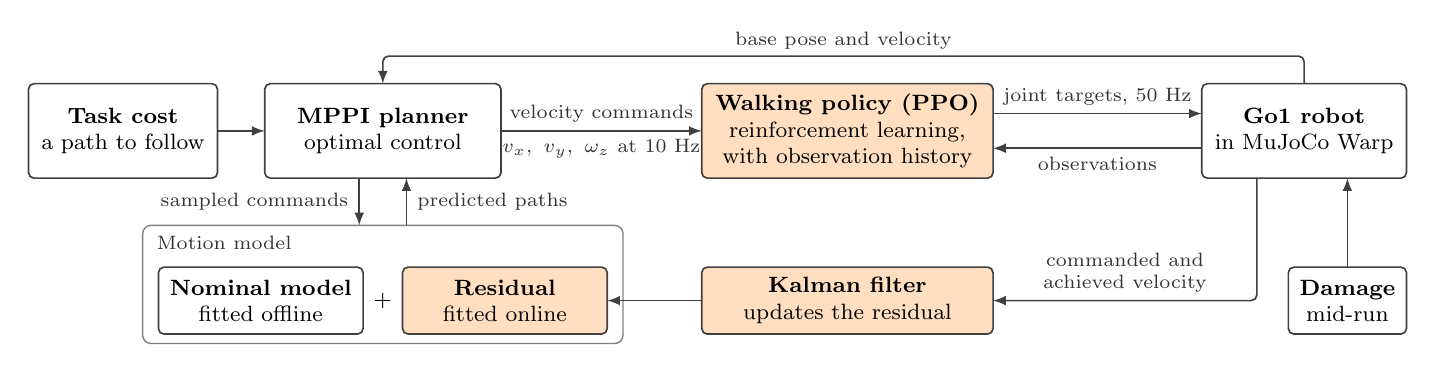
\begin{tikzpicture}[
      x=1cm, y=1cm,
      font=\footnotesize,
      box/.style={draw=black!75, line width=0.6pt, rounded corners=2pt,
        align=center, inner sep=2pt},
      adapts/.style={fill=orange!25},
      flow/.style={-latex, draw=black!75, line width=0.6pt, rounded corners=2pt},
      lab/.style={font=\scriptsize, text=black!80, align=center, inner sep=1.5pt},
    ]
    % The planner's motion model: a fixed part and a part fitted online.
    \draw[black!50, line width=0.5pt, rounded corners=3pt] (1.45, 0) rectangle (7.55, 1.5);
    \node[lab, anchor=north west] at (1.57, 1.42) {Motion model};
    \node at (4.5, 0.545) {$+$};

    % Boxes. The upper row is the control chain, left to right.
    \node[box, minimum width=2.4cm, minimum height=1.2cm] (task) at (1.2, 2.7) {\textbf{Task cost}\\a path to follow};
    \node[box, minimum width=3cm, minimum height=1.2cm] (mppi) at (4.5, 2.7) {\textbf{MPPI planner}\\optimal control};
    \node[box, adapts, minimum width=3.7cm, minimum height=1.2cm] (policy) at (10.4, 2.7) {\textbf{Walking policy (PPO)}\\reinforcement learning,\\with observation history};
    \node[box, minimum width=2.6cm, minimum height=1.2cm] (robot) at (16.2, 2.7) {\textbf{Go1 robot}\\in MuJoCo Warp};
    \node[box, minimum width=2.6cm, minimum height=0.85cm] (nominal) at (2.95, 0.545) {\textbf{Nominal model}\\fitted offline};
    \node[box, adapts, minimum width=2.6cm, minimum height=0.85cm] (residual) at (6.05, 0.545) {\textbf{Residual}\\fitted online};
    \node[box, adapts, minimum width=3.7cm, minimum height=0.85cm] (kalman) at (10.4, 0.545) {\textbf{Kalman filter}\\updates the residual};
    \node[box, minimum width=1.5cm, minimum height=0.85cm] (damage) at (16.75, 0.545) {\textbf{Damage}\\mid-run};

    % Arrows.
    \draw[flow] (2.4, 2.7) -- (3, 2.7);
    \draw[flow] (6, 2.7) -- (8.55, 2.7);
    \draw[flow] (12.25, 2.92) -- (14.9, 2.92);
    \draw[flow] (14.9, 2.48) -- (12.25, 2.48);
    \draw[flow] (4.2, 2.1) -- (4.2, 1.5);
    \draw[flow] (4.8, 1.5) -- (4.8, 2.1);
    \draw[flow] (16.2, 3.3) -- (16.2, 3.65) -- (4.5, 3.65) -- (4.5, 3.3);
    \draw[flow] (15.6, 2.1) -- (15.6, 0.545) -- (12.25, 0.545);
    \draw[flow] (8.55, 0.545) -- (7.35, 0.545);
    \draw[flow] (16.75, 0.97) -- (16.75, 2.1);

    % Arrow labels.
    \node[lab, anchor=south] at (7.275, 2.75) {velocity commands};
    \node[lab, anchor=north] at (7.275, 2.65) {$v_x,\ v_y,\ \omega_z$ at 10 Hz};
    \node[lab, anchor=south] at (13.575, 2.97) {joint targets, 50 Hz};
    \node[lab, anchor=north] at (13.575, 2.43) {observations};
    \node[lab, anchor=east] at (4.12, 1.8) {sampled commands};
    \node[lab, anchor=west] at (4.88, 1.8) {predicted paths};
    \node[lab, anchor=south] at (10.35, 3.68) {base pose and velocity};
    \node[lab, anchor=south] at (13.925, 0.595) {commanded and\\achieved velocity};
  \end{tikzpicture}\\[3pt]
  {\small\textbf{Figure 1.} The system. Shaded parts adapt online: the policy
  through its history, the planner through its residual.}
\end{center}

\section{Tools}

\begin{itemize}
  \item \textbf{Simulator:} MuJoCo Warp, the GPU-parallel version of MuJoCo,
    through the mjlab framework~\cite{mjlab}.
  \item \textbf{Existing code:} mjlab's Go1 velocity-tracking task on flat
    terrain, its PPO trainer (RSL-RL), its mid-episode events and
    randomization terms (motor gains and torque limits for the damage,
    friction and external forces for the tests), and its observation history.
    The planner and its models are our own code.
  \item \textbf{Compute:} one RTX 5080. 10,000 PPO iterations with 4096
    parallel robots take 1~h 14~min.
\end{itemize}

\section{Algorithms}

\textbf{PPO with observation history (existing code, new training problem).}
The damage is a hidden part of the state, so a policy that sees only the
current observation can at best be robust on average. Prior work treats such
changes in dynamics as a POMDP, where conditioning on history reveals the hidden
property~\cite{ni2022recurrent, locoformer}. We will train the actor
on 0.5 to 1~s of stacked observations, across damages that start at random
times within an episode, with the true damage given only to the critic. The
policy can then adapt in its forward pass, as in black-box
meta-RL~\cite{rl2}.

\textbf{MPPI (ours).} Every 0.1~s MPPI samples 2048 command sequences around
its previous plan over a 1~s horizon, rolls them through the motion model, and
scores each with a task cost $J_k$ (penalties for leaving the course and for
abrupt commands, minus progress along it). The plan moves to the average of
the samples weighted by
$w_k \propto \exp\bigl(-(J_k - J_{\min}) / (\lambda \sigma_J)\bigr)$, with
temperature $\lambda$ and $\sigma_J$ the standard deviation of the costs. Each
plan runs four such rounds.

\textbf{Motion model (ours).} The nominal model predicts the body-frame
velocity $v$ over the next plan step from the command $u$:
$v_{t+1} = A v_t + B u_t + G\, s(u_t) + c$, where $s(u)$ holds the products
$u_i |u_j|$, which capture the weaker response near the speed limits. It is
fitted once per policy by least squares on data from 409 simulated robots.

\textbf{Online residual (ours, the planner's adaptation).} Following
Neural-Fly~\cite{neuralfly}, the nominal model stays fixed and we add a
residual that is linear in a few coefficients:
$v_{t+1} = f_{\mathrm{nom}}(v_t, u_t) + \Phi(v_t, u_t)\, a_t$. At every plan
step a Kalman filter updates the 3 to 12 coefficients $a_t$ from the nominal
model's latest prediction error, with a leak that pulls them back toward zero.
We start with hand-chosen features $\Phi$ (an offset per axis, which is a
disturbance observer, and gains on the commands) and will then learn $\Phi$
offline from motion under many damages, as Neural-Fly does.

\section{Planned work, experiments and expected results}

\textbf{Planned work.} (1) A mid-episode damage event that scales down motor
gains or torque limits on one leg, down to zero for a dead motor (any joint,
any severity, up to the whole leg), with some combinations held out of
training. (2) PPO policies without and with history, trained identically on
the same damages. (3) A course with turns in both directions, as an MPPI cost.
(4) A residual that is stable when a change starts
(Section~\ref{sec:prelim}), then learned features. (5) The evaluation and a
demo video. (6) As a stretch goal, a joint-level residual as an input to the
policy.

\textbf{Experiments.} Four controllers face the same damages, with the same
MPPI, cost and command limits: (1) no history and a fixed planner model, (2)
history only, (3) online residual only, (4) both (ours). We will run 50 trials
per controller and damage and report, with confidence intervals, three groups:
damages seen in training, held-out damages, and kinds of change never trained
on (a payload, friction below the trained range). The measures are recovery
time (until velocity tracking is back within a tolerance), path error, falls,
and time to finish. We will also plot the residual's coefficients around the
damage and compare three feature sets: offset, offset plus gains, learned.

\textbf{Expected results.} (i) The policy with history regains a steady gait
within about 2~s and tracks commands better after damage than the policy
without history, also on held-out damages. (ii) The residual lowers path error
on damages that leave a lower top speed or a steady drift. Our first test
points this way (Section~\ref{sec:prelim}). (iii) The combination has the
lowest path error. Two risks: the levels may overlap (if the policy
compensates almost fully, the residual adds little), and the residual can
destabilize the planner, as it did with 12 coefficients
(Section~\ref{sec:prelim}).

\section{Preliminary work}
\label{sec:prelim}

All results below use a policy trained without damage or history; those two
parts are not started.
\begin{itemize}
  \item \textbf{Motion model:} predicting 2~s ahead on held-out robots, its
    mean position error is 0.15~m, against 0.27~m for a model that assumes the
    robot moves exactly as commanded (they travel 1.24~m on average).
  \item \textbf{MPPI demos:} (i) a race around a circular track of radius
    2.5~m: 5.5~s laps, no falls, 6 to 8~ms per plan; (ii) pushing a box
    through three goals, planning in 384 parallel simulations at a quarter of
    real time.
  \item \textbf{Online residual:} implemented and unit-tested. On synthetic
    data with a known change, the 12-coefficient version removes 51 to 64\% of
    the added model error in the first second and 72 to 89\% in the next. In
    the simulator, a steady 30~N pulled the robot outward during the circle
    race (ten 30~s runs per row, pull from 8~s on):
\end{itemize}
\begin{center}
  \small
  \begin{tabular}{@{}lll@{}}
    \toprule
    Planner's model & Falls & Off the track during the pull: median (range) \\
    \midrule
    Fixed, no adaptation & 0 of 10 & 90\% (87 to 92\%) \\
    Residual, offset per axis (3 coefficients) & 0 of 10 & 0\% (0 to 4\%) \\
    Residual, diagonal gains and offset (6) & 0 of 10 & 0\% (0 to 3\%) \\
    Residual, $3 \times 3$ gains and offset (12) & 2 of 10 & 0\% (0 to 20\%) in
    the runs without a fall \\
    \bottomrule
  \end{tabular}
\end{center}
With the residual the robot stays on the track, at a cost before the pull: the
3- and 6-coefficient versions cross the inside edge 20 to 30\% of the time, by
up to 8~cm, unlike the fixed model. With 12 coefficients the planner brakes
hard and swings its commands when the pull starts, and the robot fell
in two runs. The likely cause: with constant commands, a steady pull looks
like a drift that grows with speed. A steady pull is also easier than leg
damage.

{\footnotesize
% Tighter reference list, as in the hand-written version.
\let\oldthebibliography\thebibliography
\renewcommand{\thebibliography}[1]{\oldthebibliography{#1}%
  \setlength{\itemsep}{0pt}\setlength{\parskip}{0pt}}
\bibliographystyle{unsrt}
\bibliography{references}
}

\end{document}
